
% # COPYRIGHT:
%
%   Copyright (C)  2011 Jeremiah Mahler <jmmahler@gmail.com>.
%   Permission is granted to copy, distribute and/or modify this document
%   under the terms of the GNU Free Documentation License, Version 1.3
%   or any later version published by the Free Software Foundation;
%   with no Invariant Sections, no Front-Cover Texts, and no Back-Cover Texts.
%   A copy of the license is included in the file "fdl-1.3.txt".
%

\documentclass[12pt]{article}
%\documentclass[10pt]{article}

%\usepackage{mslapa}
\usepackage{hyperref}
\usepackage{amsmath}
\usepackage{graphicx}
\usepackage{ulem}
%\usepackage{vmargin}
\usepackage{tabularx}
\usepackage{sectsty}
\usepackage{pbox}
\usepackage{bigstrut}
\usepackage{enumerate}
\usepackage{parskip}  % add spaces between paragraphs

%\usepackage{cleveref}

%\setpapersize{USletter}
\sectionfont{\normalsize}
\subsectionfont{\normalsize}

% configure \bigstrut size
% This configures spacing above and below rows in a tabularx.
%\renewcommand{\bigstrutjot}{6pt}
\renewcommand{\bigstrutjot}{2.0\jot}

\setlength{\parindent}{0in}

\raggedright

\begin{document}

% {{{ Cover Page

\centerline{\bf EECE 144}
\centerline{\bf Fall 2011}
\centerline{\bf}
\centerline{\bf Lab Report \#4}
\centerline{\bf Section 4}
\centerline{\bf 9/28/2011}

% signature area
\begin{center}
\begin{tabularx}{\textwidth}[b]{X l l}
Submitted by: & & \\
Signature & Printed Name & Date \\
\hline
\multicolumn{1}{|X|}{} & \multicolumn{1}{|l|}{\bigstrut \bf Jeremiah Mahler} & \multicolumn{1}{|l|}{\bf Sep 28, 2011} \\
\hline
\multicolumn{1}{|X|}{} & \multicolumn{1}{|l|}{\bigstrut \bf Marvanee Johnson} & \multicolumn{1}{|l|}{\bf Sep 28, 2011} \\
\hline
\end{tabularx}
\end{center}
% }}}

\section{Description/Objectives}

The objective of this lab is to derive the equivalent versions
of a logic function in both the minterm canonical SOP
form and the maxterm canonical POS form.
And then implement both of these versions in hardware and
verify their outputs.

\section{Procedure}
\label{sec:plan}

The minterm canonical SOP form for the logic function used in this
experiment is given in Equation \ref{eq:minsop}.
The equivalent maxterm canonical POS form is given in Equation \ref{eq:maxpos}.
Both functions produce an equivalent truth table as given in Figure \ref{fig:tt1}.
%\nocite{roth2009fundamentals}

\begin{align}
f(x, y) &= \sum m(0, 2) \label{eq:minsop} \\
	    &= m_0 + m_2 \notag \\
		&= x' y' + x y' \notag
\end{align}

\begin{align}
f(x, y) &= \prod M(1, 3) \label{eq:maxpos} \\
	 &= M_1 M_3 \notag \\
	 &= (x + y')(x' + y') \notag
\end{align}

\begin{figure}[!hbt]
\center
\begin{tabular}[t]{| l | l | l |}
\hline
$x$ & $y$ & $f(x, y)$\\
\hline
0 & 0 & 1 \\
\hline
0 & 1 & 0 \\
\hline
1 & 0 & 1 \\
\hline
1 & 1 & 0 \\
\hline
\end{tabular}

\caption{Truth table of the equivalent functions in Equation \ref{eq:minsop} and \ref{eq:maxpos}.}
\label{fig:tt1}
\end{figure}

The design of these logic functions implemented with gates is shown
in Figure \ref{fig:minsoplog} and \ref{fig:maxposlog}.
Interestingly, the only change made between the two diagrams is
that of swapping the AND gates with OR gates and vice versa.

\begin{figure}[!hbtp]
\center
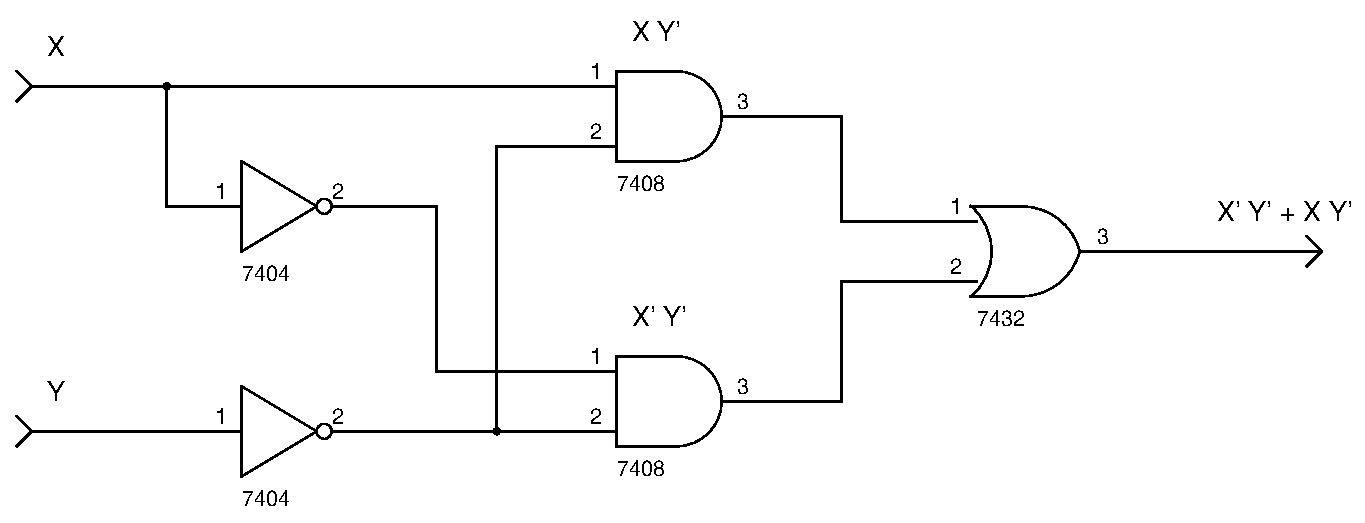
\includegraphics[scale=0.5]{minsop-01}
\caption{Diagram of equation \ref{eq:minsop}; minterm canonical SOP form.}
\label{fig:minsoplog}
\end{figure}

\begin{figure}[!hbtp]
\center
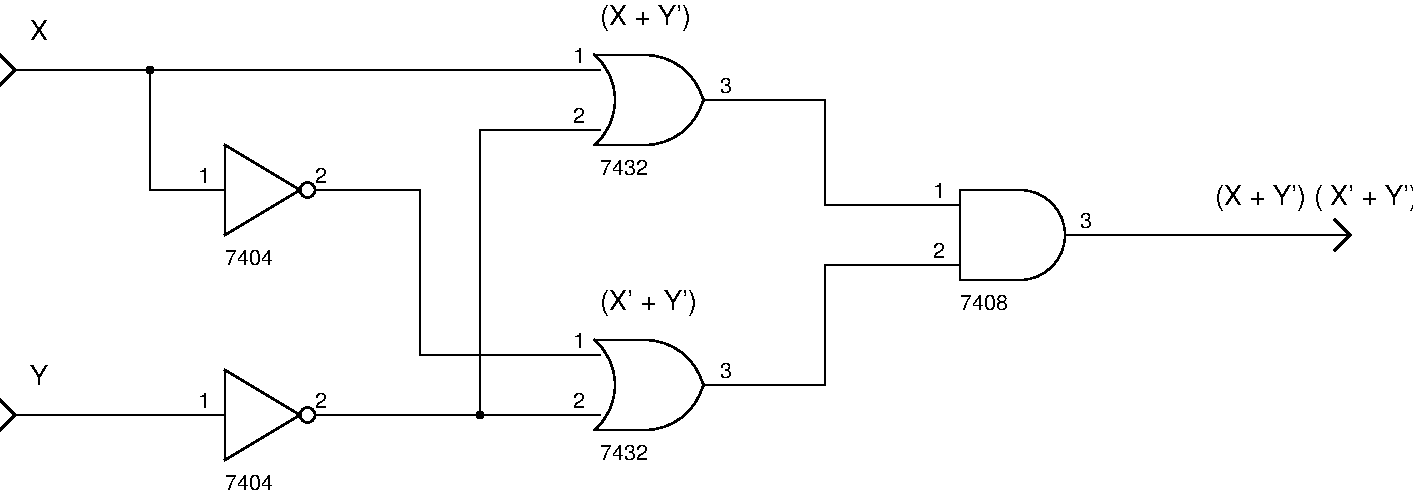
\includegraphics[scale=0.5]{maxpos-01}
\caption{Diagram of equation \ref{eq:maxpos}; maxterm canonical POS form.}
\label{fig:maxposlog}
\end{figure}

\clearpage

\subsection{Wiring}

To wire the chips it is necessary to have all the pertinent data sheets.
These describe the function of each pin, the voltage characteristics and
the orientation of the pins.
The general procedure is as follows:
\begin{itemize}
	\item Choose a subset of the circuit to implement from Figure \ref{fig:minsoplog} or Figure \ref{fig:maxposlog}..
	\item Refer to the data sheet for the pin identification of the chip involved.
	\item Connect wires.
	\item Repeat until all subsets of the circuit have been implemented.
\end{itemize}

As an example, the diagram (Figure \ref{fig:minsoplog}) showed that
each pin was connected to the NOT gates first.
So the first step was to connect each of the switches which represented
the inputs $x$ and $y$ to the corresponding pins on the 7404 NOT gate chip.

The final output should be connected to an LED along with a resistor
that limits the current to no more than 20 mA.
Be sure to use pull down resistors on the mechanical switch inputs to
guarantee a near 0 volt logic low.
A 1k pull down resistor works correctly in most cases.

%\clearpage

\section{Observations}

The output of each logic function implemented in hardware agreed
with the truth table.
To switch between the minterm POS to maxterm SOP it was only
necessary to swap the 7432 OR gate with the 7408 AND gate.
This is possible because the layouts are identical for each chip.

\clearpage
\section{Conclusion}

This lab was a success in showing the equivalence of minterm SOP
form and maxterm POS form by implementing the function in hardware.

% flush all the figures
%\clearpage

%\pagebreak
%\renewcommand*{\refname}{\vspace{-8mm}}
%\section{References}
%\bibliographystyle{plain}
%\bibliographystyle{mslapa}
%\bibliographystyle{ieeetr}
%\bibliography{../references}

% Appendix (if needed)

\end{document}

% vim:foldmethod=marker
